\documentclass{article}[18pt]
\usepackage[utf8]{inputenc}
\usepackage[margin=0.7in]{geometry}
\usepackage{parselines} 
\usepackage{amsmath}
\usepackage{titlesec}
\usepackage{pgfplots}
\usepackage{graphicx}
\usepackage[english]{babel}
\usepackage{fancyhdr}
\usepackage{amssymb}
\pgfplotsset{width=10cm,compat=1.9}
\usepackage{mwe}
\usepackage{float}
\usepackage{polynom}
\usepackage{relsize}
\usepackage{tikz}
\usepackage{tikz-3dplot} %requires 3dplot.sty to be in same directory, or in your LaTeX installation
\usepackage{mathtools}
\usetikzlibrary{calc,quotes,angles}
\titlespacing\section{0pt}{14pt plus 4pt minus 2pt}{0pt plus 2pt minus 2pt}
\newlength\tindent
\setlength{\tindent}{\parindent}
\setlength{\parindent}{0pt}
\renewcommand{\indent}{\hspace*{\tindent}}

\pagestyle{fancy}
\fancyhf{}
\rhead{Sam Robbins 13SE}
\lhead{A Level Maths - C4}
\rfoot{Page \thepage}

\newcommand{\R}{\mathbb{R}}
\pgfplotsset{ytick style={draw=none}}
\pgfplotsset{xtick style={draw=none}}

\begin{document}
\begin{center}
\underline{\huge Differentiation}
\end{center}
\section{3D Vectors}
\tdplotsetmaincoords{60}{110}
\pgfmathsetmacro{\rvec}{.8}
\pgfmathsetmacro{\thetavec}{30}
\pgfmathsetmacro{\phivec}{60}
\begin{tikzpicture}[scale=5,tdplot_main_coords]

\coordinate (O) at (0,0,0);

\tdplotsetcoord{P}{1.5*\rvec}{1.5*\thetavec}{1.5*\phivec}

\draw[thick,->] (0,0,0) -- (-1,0,0) node[anchor=north west]{$z$};
\draw[thick,->] (0,0,0) -- (0,1,0) node[anchor=north west]{$x$};
\draw[thick,->] (0,0,0) -- (0,0,1) node[anchor=south]{$y$};

\draw[-stealth,color=red] (O) -- (P) node[anchor=west,above] {A(x,y,z)} node[midway,anchor=east,above]{\textbf{a}};
\end{tikzpicture}
\\
\\
$\overrightarrow{OA}=xi+yj+zk$\\
\\
$\overrightarrow{OA}=\begin{pmatrix}x\\y\\z\end{pmatrix}$\\
\\
\\
\textbf{Magnitude of $\mathbf{\overrightarrow{OA}}$}\\
\\
$|\overrightarrow{OA}|=\sqrt{x^2+y^2+z^2}$\\
\\
\textbf{The vector between two vectors}\\
\\
$\overrightarrow{OA}=\begin{pmatrix}
x_1\\
y_1\\
z_1\\
\end{pmatrix}
\quad
\overrightarrow{OB}=\begin{pmatrix}
x_2\\
y_2\\
z_2\\
\end{pmatrix}
$\\
\\
\\
$|\overrightarrow{AB}|=\sqrt{(x_2-x_1)^2+(y_2-y_1)^2+(z_2-z_1)^2}$\\
\\
\newpage
\section{Vector dot product}
$\mathbf{a}=\begin{pmatrix}
x_1\\
y_1\\
z_1\\
\end{pmatrix}
\quad
\mathbf{b}=\begin{pmatrix}
x_2\\
y_2\\
z_2\\
\end{pmatrix}
$
\\
\\
$\mathbf{a}\mathlarger{\cdot}\mathbf{b}=x_1x_2+y_1y_2+z_1z_2$\\
\\
\\

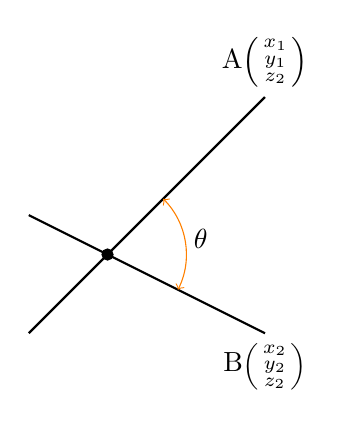
\begin{tikzpicture}
\coordinate (a) at (0,0);
\coordinate (b) at (1,-0.5);
\coordinate (c) at (2,2);
\draw[black, thick] (-1,0.5) -- (2,-1) node[below] {B$\mathsmaller{\begin{psmallmatrix}
x_2\\
y_2\\
z_2\\
\end{psmallmatrix}}$};
\draw[black, thick] (-1,-1) -- (2,2) node[above] 
{A$\begin{psmallmatrix}
x_1\\
y_1\\
z_2\\
\end{psmallmatrix}
$}
;
\filldraw[black] (0,0) circle (2pt);

\draw pic["$\theta$",draw=orange,<->,angle eccentricity=1.2,angle radius=1cm] {angle=b--a--c};
\end{tikzpicture}
\\
\\
$\cos\theta=\dfrac{\mathbf{a}\cdot \mathbf{b}}{|\mathbf{a}||\mathbf{b}|}$\\
\\
\subsection{Perpendicular vectors}
$\cos 90=0$\\
\\
$\cos\theta=\dfrac{\mathbf{a}\cdot \mathbf{b}}{|\mathbf{a}||\mathbf{b}|}$\\
\\
$\mathbf{a}\cdot \mathbf{b}=0$
\\
\subsection{Parallel vectors}
$\theta=1 \quad \cos\theta=1$\\
\\
$\mathbf{a}\cdot \mathbf{b}=|\mathbf{a}||\mathbf{b}|$
\\
\section{Vector equation of a straight line}
Types of situation:\\
\\
\textbf{1. Through one point parallel to a given vector}\\
\\
\textit{Find the equation of the line through \textbf{a} which is parallel to \textbf{b}}\\
\\
\textcolor{red}{\textbf{r}=\textbf{a}+t\textbf{b}}\\
\\
\textbf{2. A line through two points}\\
\\
\textit{Find the equation of a line through a and b}\\
\\
\textcolor{red}{$\mathbf{r}=\mathbf{a}+t(\mathbf{b-a})$}\\
\\
\section{Proofs involving vectors}
\subsection{Example of proving a point lies on a vector line}
\textit{Show that} $\begin{pmatrix}
9\\
9\\
3\\
\end{pmatrix}
$ lies on the line \textbf{r}=$\begin{pmatrix}
1\\
4\\
2\\
\end{pmatrix}+\lambda\begin{pmatrix}
8\\
5\\
1\\
\end{pmatrix}$\\
\\
\textbf{Substitute the point equalling r}\\
\\
$\begin{pmatrix}
9\\
9\\
3\\
\end{pmatrix}
=
\begin{pmatrix}
1\\
4\\
2\\
\end{pmatrix}+\lambda
\begin{pmatrix}
8\\
5\\
1\\
\end{pmatrix}$
\\
This is true when $\lambda$ equals one so the point is on the line
\subsection{Example of finding where two lines intersect}
\textit{Where do the lines $L_1$ and $L_2$ intersect}\\
\\
$L_1: \mathbf{r}=
\begin{pmatrix}
3\\
1\\
2\\
\end{pmatrix}+\lambda
\begin{pmatrix}
1\\
-1\\
4\\
\end{pmatrix}$\\
\\
\\
$L_2: \mathbf{r}=
\begin{pmatrix}
0\\
4\\
-2\\
\end{pmatrix}+\mu
\begin{pmatrix}
1\\
1\\
0\\
\end{pmatrix}$\\
\\
\textbf{Equal coordinates in a certain dimension to each other, preferably where constants can be eliminated}\\
\\
$2+4\lambda=-2$\\
\\
$\lambda=-1$
\section{Finding the angle between two straight lines}
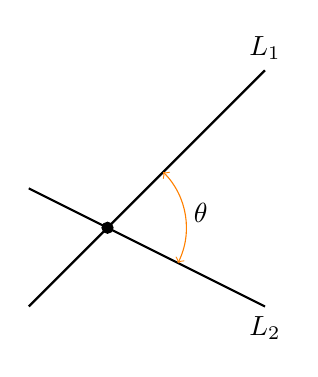
\begin{tikzpicture}
\coordinate (a) at (0,0);
\coordinate (b) at (1,-0.5);
\coordinate (c) at (2,2);
\draw[black, thick] (-1,0.5) -- (2,-1) node[below] {$L_2$};
\draw[black, thick] (-1,-1) -- (2,2) node[above] 
{$L_1$}
;
\filldraw[black] (0,0) circle (2pt);

\draw pic["$\theta$",draw=orange,<->,angle eccentricity=1.2,angle radius=1cm] {angle=b--a--c};
\end{tikzpicture}
\\
These vectors can be represented in the form $\mathbf{r}=\mathbf{a}+\lambda\mathbf{d_1}$\\
\\
\textbf{Example}\\
\\
$\mathbf{r}=
\begin{pmatrix}
2\\
0\\
1\\
\end{pmatrix}
+\lambda
\begin{pmatrix}
11\\
5\\
3\\
\end{pmatrix}$\\
\\
Here $\mathbf{d_1}$ is $\begin{pmatrix}
11\\
5\\
3\\
\end{pmatrix}$\\
\\
\\
$\cos\theta=\Bigg|\dfrac{\mathbf{d_1}\cdot\mathbf{d_2}}{|\mathbf{d_1}||\mathbf{d_2}|}\Bigg|$
\\
\section{Problems involving points on vector lines and perpendicular problems}
\begin{tikzpicture}
\coordinate (a) at (0,0);
\coordinate (b) at (1,-1);
\coordinate (c) at (2,2);
\draw[black, thick] (-1,1) -- (2,-2) node[below] {O};
\draw[black, thick] (-1,-1) -- (2,2) node[above] 
{$L_1$}
;
\filldraw[black] (0,0) circle (2pt);

\draw[black, thick] (0,0) -- (0.3,-0.3) -- (0.6,0) -- (0.3,0.3) -- cycle;
\node[text width=4cm] at (1.6,-0.7) {$\begin{psmallmatrix}
x\\
y\\
z\\
\end{psmallmatrix}
$};
\end{tikzpicture}\\
$L_1: \mathbf{r}=
\begin{pmatrix}
9\\
-2\\
1\\
\end{pmatrix}+\lambda
\begin{pmatrix}
-3\\
4\\
5\\
\end{pmatrix}$\\
\\
\\
$\begin{pmatrix}
x\\
y\\
z\\
\end{pmatrix}=
\begin{pmatrix}
9\\
-2\\
1\\
\end{pmatrix}+\lambda
\begin{pmatrix}
-3\\
4\\
5\\
\end{pmatrix}$
\\
\\
Using the vector dot product $a\cdot b=0$ we can find the coordinates of X\\
\\
$\overrightarrow{OX}\cdot \mathbf{d}=0$\\
\\
$\begin{pmatrix}
9-3\lambda\\
-2+4\lambda\\
1+5\lambda
\end{pmatrix}\cdot
\begin{pmatrix}
-3\\
4\\
5\\
\end{pmatrix}=0$
\\
\\
$\lambda=\dfrac{3}{5}$
\end{document}